During your lab period, the TAs will guide the class through the first modifications to the starter code that you must make, described in this section.
If you do not attend your lab period, then you must complete this section on your own.
\textbf{\textit{Except during lab time, you may }not\textit{ discuss the solutions for this section with other students.}}


\subsection{Reviewing the Datasheet}

Read the Datasheet section that discusses \href{https://cow-pi.readthedocs.io/en/latest/CowPi_\lowercaseprocessor/io_registers.html#interrupts}{Interrupts}, and review the \href{https://cow-pi.readthedocs.io/en/latest/CowPi_\lowercaseprocessor/io_registers.html#timers}{Timers} section.

%You can skip over the section that covers registering external interrupt handlers using \function{attachInterrupt()}, as we will use pin change interrupts.
%You can skip over the section that covers the timers ``Normal'' mode, as we will use ``Clear Timer on Compare'' (CTC) mode.
%You can skip over the section that covers configuring TIMER0, as we will use only TIMER1 and TIMER2.

You can skip over the section that discusses the use of \function{attachInterrupt()}, as we will use \function{register_pin_ISR()}.
The discussion of \function{cowpi_register_pin_ISR()} is relevant, as \function{register_pin_ISR()} in \textit{interrupt\_support.cpp} has the same signature and exhibits the same behavior.

Review the header comments in \textit{interrupt\_support.h}.
\ifdefstring{\processor}{ATmega328P}{
    We will use the \function{configure_timer()} function to configure two timers to fire periodic interrupts,
    and we will use the \function{register_timer_ISR()} function to register interrupt handlers for those interupts.
    \textit{You will} not \textit{need to explicitly set the timer registers' bits as described in the datasheet};
    however, familiarizing yourself with the timers' limitations might be helpful.
}{}
\ifdefstring{\processor}{RP2040}{
    We will use the \function{register_timer_ISR()} function to configure two timers to fire periodic interrupts
    and to register interrupt handlers for those interupts.
    \textit{You will} not \textit{need to explicitly set the timer registers' bits,
        nor will you need to directly invoke any MBED~OS functions.}
}{}


\subsection{Examining the Starter Code}

Familiarize yourself with the functions in \requiredfiles, and the header comments that describe what the functions will do.

\subsection{Debouncing} \label{subsec:debouncing}

\begin{figure}[h]
    \centering
    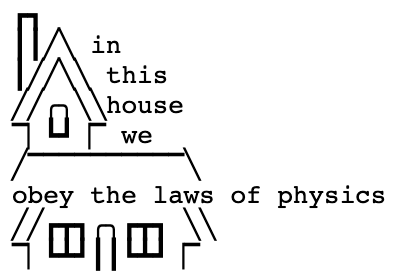
\includegraphics[height=3.5cm]{in-this-house}
\end{figure}

Mechanical buttons and switches demonstrate a phenomenon called \textit{switch bounce}.
This causes voltage to fluctuate for hundreds, often thousands, of microseconds when the contacts close or open.
When this fluctuation is in the indeterminate region between the logical low and high thresholds, it can cause the logic level to ``bounce'' back-and-forth between high and low until settling into the final, correct logic level.
This causes the digital circuitry or software to ``see'' multiple triggering events.

A traditional way to debounce is to introduce a simple low-pass filter using a resistor and a capacitor.
Other common hardware-based approaches use digital feedback circuits.
Hardware design can be simplified, and manufacturing cost can be reduced, by solving a hardware problem with software.
This, of course, transfers the design complexity to the software.

The CowPi library includes the \function{cowpi_debounce_byte()}, \function{cowpi_debounce_short()}, and \function{cowpi_debounce_long()}  functions that essentially implement a low-pass filter in software.
The functions in \textit{io\_functions.c} make use of \function{cowpi_debounce_byte()}\ifdefstring{\processor}{RP2040}{ and \function{cowpi_debounce_long()}}{}.
When you modify these functions, as long as you preserve those \function{cowpi_debounce_byte()} calls, you do not need to worry further about debouncing.


\subsection{Handling Key Presses}

% TODO: figure out how to parameterize the interplay between interrupts and the specific application

\subsubsection{The Interrupt Service Routine}

In \textit{inputs.c}, locate the \function{initialize_interrupts()} function.
In this function:
\begin{description}
%    \item Use \function{cowpi_register_pin_ISR()} to register \function{handle_keypress()} as the interrupt service routine that should be invoked whenever there is key movement on the keypad.
    \checkoffitem{Use \function{register_pin_ISR()} to register \function{handle_keypress()} as the interrupt service routine that should be invoked whenever there is key movement on the keypad.}
\end{description}

\paragraph{Hint} Which microcontroller pins did you use to detect key presses in PollingLab?
\paragraph{Important} When you provide the name of the ISR, provide \textit{only} the name -- do \textit{not} include parentheses!
\begin{itemize}
    \item With the parentheses, you are saying that the function should execute \textit{now} and the result is the argument you're providing
    \item Without the parentheses, you are passing a \textit{function pointer}, which is what is needed here \\
\end{itemize}

Locate the \function{handle_keypress()} function.

After the busy-wait loop terminates, the \lstinline{key} variable holds the character corresponding to the key that was pressed, or \lstinline{'\0'} if no key was pressed (\textit{i.e.}, a key was released).
\begin{description}
    \checkoffitem{Add code that will call the \function{update_character()} function if a key was pressed.}
\end{description}

\subsubsection{The Logic} \label{subsubsec:logic}

In \textit{character\_selector.c}, locate the \lstinline{characters} and \lstinline{key_modulus} arrays.
The \lstinline{characters} nested array describes the characters that can be produced by cycling through each of the numeric keys on the keypad.\footnote{
    An underscore character (`\_') is used in place of a space character so that it's more clear on the display module whether a blank at the end of the message is meant to be a space or is merely an empty blank.
}
The \lstinline{key_modules} array describes how many useful characters are in each of \lstinline{characters}' rows.\footnote{
    Because \lstinline{characters} is a nested array, all rows occupy 5 bytes, even though most rows don't have five useful characters.
}

The \lstinline{working_key} global variable selects the \lstinline{characters} row, and the \lstinline{character_index} global variable selects the column.
The \function{reset_selector()} function sets both of these variables to -1, using named constants to provide meaning to these special values.

Locate the \function{update_character()} function in \textit{character\_selector.c}.
In this function:
\begin{description}
    \checkoffitem{Determine if the input is valid.}
    \checkoffitem{If so:}
    \begin{description}
        \checkoffitem{Determine what the first character should be, according to Requirements~\ref{spec:keypad} and \ref{spec:firstPress}, and}
        \checkoffitem{Send that character to the message editor using the \function{replace_character()} function.}
    \end{description}
\end{description}
(The \function{update_character()} function will have more responsibility later,
but for now, just focus on sending a character to the message editor.)

In \textit{message\_editor.c}, locate the \lstinline{message} array and related variables.
The \lstinline{message} array is a buffer to store the message being edited,
and \lstinline{message_index} is used to track the end of the message.
The \lstinline{display_start} pointer is used to indicate the start of the substring that will be displayed on the display module.

Locate the \function{replace_character()} function in \textit{message\_editor.c}.
In this function:
\begin{description}
    \checkoffitem{Add code to place the character in the \lstinline{message} buffer at \lstinline{message_index}.
    Do \textit{not} update \lstinline{message_index}.}
\end{description}
(You will make further changes to the \function{replace_character()} function later,
but for now, just focus placing the character at the end of the string.)

\subsubsection{Test Your Code}

At this point, all characters are placed at the start of the message, but you can still check:
\begin{description}
%    \item Does your code cycle through the characters for each key?
    \checkoffitem{Does your code produce the first character from each number key's character sequence?}
    \checkoffitem{Does your code produce characters for all the number keys?}
    \checkoffitem{Does your code produce characters for only the number keys?}
\end{description}


\subsection{Blinking the LED} \label{subsec:blinking}

According to Requirement~\ref{spec:pressIndicator}, the right LED needs to blink for approximately \textonequarter\ second whenever the user presses a key.

In \textit{inputs.c}, locate the \lstinline{#define LED_TIMER} macro and the \lstinline{supplemental_counter} variable.
We will use \lstinline{LED_TIMER} as a handle for a specific timer when calling
\ifdefstring{\processor}{ATmega328P}{\function{configure_timer()}, as well as}{}
\function{register_timer_ISR()} and \function{reset_timer()}.
\ifdefstring{\processor}{ATmega328P}{Specifically, these functions will it to configure the ATmega328P's TIMER2 and to register and ISR for interrupts generated by TIMER2.}{}

\ifdefstring{\processor}{ATmega328P}{
    Unfortunately, the greatest interrupt period possible for TIMER2 is 16,384\textmu s (16.384ms), well short of \textonequarter second.
    Our solution to this is
}{}
\ifdefstring{\processor}{RP2040}{
    While we \textit{can} configure a timer for 250,000\textmu s (250ms), we won't.
    Instead, our solution will be
}{}
to approximate \textonequarter s as 256ms, configure the timer for a factor of 256ms, and then use \lstinline{supplemental_counter} to count the number of times that the timer fires an interrupt.
When and only when \lstinline{supplemental_counter}'s value indicates that 256ms has passed, we will take further action.
\ifdefstring{\processor}{RP2040}{
    This probably seems like a roundabout solution -- all else being equal, it is! -- however,
    if the time between actions is variable (as might be the case in the group project) then this technique will simplify your solution.
    You might as well get familiar with the technique now, in the simpler case of the time between actions holding constant.
}{}

\subsubsection{Configuring the Timer}

We will approximate \textonequarter second as 256ms.
The reason for this is that we want our ISRs to execute as fast as possible, and if we tried to take action after exactly 250ms, we will have to resort to division,
\ifdefstring{\processor}{ATmega328P}{which takes hundreds of cycles on the ATmega328P microcontroller.}{}
\ifdefstring{\processor}{RP2040}{which isn't terribly slow on the RP2040 (it has an 8-cycle integer divider); however, it isn't as fast as using a bitwise operation.}{}
If we choose to take action after 256ms, then we can select a power-of-two, $2^n$ such that the ISR takes action once every $2^n$ times that the ISR runs.
Now, we can determine when the ISR has run $ISR$ times by adding 1 to \lstinline{supplemental_counter} each time the ISR runs and then applying a bitmask ($(1 << n) - 1$).
This effectively will cause overflow every $2^n$ increments.

We shall set the timer's interrupt period to $\frac{256}{2^n}ms = \frac{256000}{2^n}\mu s$.
Specifically, we shall set the interrupt period to 8ms and take action when the interrupt has fired 32 times.


In \function{initialize_interrupts()}:
\begin{description}
    \checkoffitem{Use \ifdefstring{\processor}{ATmega328P}{\function{configure_timer()} and}{} \function{register_timer_ISR()} to configure the \lstinline{LED_TIMER} to generate an interrupt every 8,000\textmu s and to register \function{handle_led_timer()} as its ISR for that interrupt.}
        \ifdefstring{\processor}{ATmega328P}{\begin{itemize}
            \item When calling \function{register_timer_ISR()}, use ISR slot 0.
        \end{itemize}}{}
\end{description}

%\begin{itemize}
%    \item Consulting the Datasheet's \href{https://cow-pi.readthedocs.io/en/latest/microcontroller.html#configuring-timer2}{Configuring TIMER2} section.
%        Assign the base address for TIMER2's registers to \lstinline{led_timer}.
%    \item Using the equation in the Datasheet's \href{https://cow-pi.readthedocs.io/en/latest/microcontroller.html#clear-timer-on-compare-mode}{Clear Timer on Compare Mode} section,
%        select a prescaler such that the resulting comparison value is at most $2^8$.
%    \item Using the Datasheet's Tables 17--19, construct a bit vector for TIMER2's control register for ``CTC'' mode with your chosen prescaler.
%        Assign this bit vector to \lstinline{led_timer}'s \lstinline{control} field.
%    \item Subtract 1 from your calculated comparison value, and assign the result to \lstinline{led_timer}'s \lstinline{compareA} field. \\
%        \textcolor{red}{IMPORTANT! The assignment to the \lstinline{compareA} field must occur \textit{after} the assignment to the \lstinline{control} register.}
%    \item Consulting the Datasheet's \href{https://cow-pi.readthedocs.io/en/latest/microcontroller.html#timer-interrupts}{Timer Interrupts} section, enable the \lstinline{TIMER2_COMPA_vect} interrupt vector by setting the \lstinline{OCIE2A} bit to 1.
%\end{itemize}
%
%In \function{reset_timers()}:
%
%\begin{itemize}
%    \item Uncomment \lstinline{led_timer->counter = 0;}
%\end{itemize}

\subsubsection{Turning the LED On and Off}

According to Requirement~\ref{spec:pressIndicator}, the right LED shall illuminate when the user presses a key.
\begin{description}
    \checkoffitem{Add a call to \function{cowpi_illuminate_right_led()} in the part of \lstinline{inputs.c} that will run when a key has been pressed.}
    \checkoffitem{Immediately after that, call \function{reset_timers()} to reset the timers' counters and to set the supplemental counter to zero.}
\end{description}

According to Requirement~\ref{spec:pressIndicator}, the right LED needs to deluminate after approximately \textonequarter\ second, which we are approximating as 256ms.
Locate the \function{handle_led_timer()} in \textit{inputs.c}.

\begin{description}
    \checkoffitem{Add code to \function{handle_led_timer()} to increment \lstinline{supplemental_counter} and to cause it to overflow after 32 increments.}
    \checkoffitem{Add code to \function{handle_led_timer()} that will call \function{cowpi_deluminate_right_led()} whenever \lstinline{supplemental_counter} overflows.}
\end{description}

You should take the time to convince yourself that the LED will turn off exactly 256ms after a key is pressed.
You should take the time to convince yourself that there will be no observable effect when \lstinline{supplemental_counter} overflows while the LED is off.


\subsubsection{Test Your Code}

The easy part of testing this code is:
\begin{description}
    \checkoffitem{When you press a key, does the right LED turn on and then off again?}
\end{description}

Testing that the LED illuminates for exactly 256ms is a bit harder to do on a human scale, but you can give yourself a sanity check.
\begin{description}
    \checkoffitem{Temporarily change \function{handle_led_timer()} to cause \lstinline{supplemental_counter} to overflow after 128 increments.}
        \begin{itemize}
            \item This will cause the LED to deluminate after 1.024ms
        \end{itemize}
    \checkoffitem{When the right LED illuminates after you press a key, does it deluminate after about a second?}
    \checkoffitem{Change \function{handle_led_timer()} back to causing \lstinline{supplemental_counter} to overflow after 32 increments.}
\end{description}

\vspace{1cm}

You are now ready to complete the remainder of this assignment on your own.
Reminders:
\begin{itemize}
    \item You can complete Sections~\ref{sec:characterGeneration} and \ref{sec:oddsAndEnds}.
    \item \collaborationrules
\end{itemize}

